\section{Threat Model, Assumptions, and Goals}
\label{sec:threat}

\begin{figure}[t]
\centering
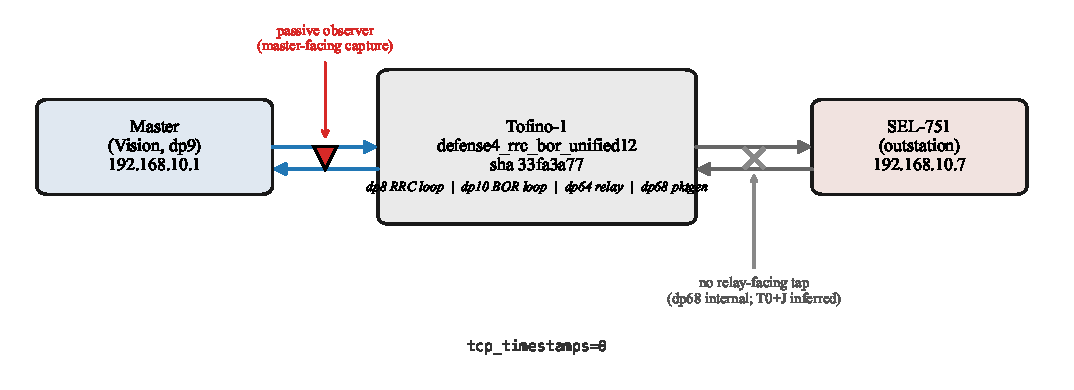
\includegraphics[width=0.98\columnwidth]{figures/fig_system}
\caption{Testbed and observation model. The master reaches the physical SEL-751 through one Tofino-1
switch. The passive adversary observes only the master-facing link; the relay-facing link and the
switch-internal loopbacks (\code{dp8} for response shaping, \code{dp10} for the control-command hold) are not observed.}
\label{fig:system}
\end{figure}

\subsection{System and observation model}
Figure~\ref{fig:system} shows the setup. We consider a DNP3-over-TCP link between one master and one
outstation, the SEL-751 relay, with a Tofino switch on the path at the outstation edge. The master polls the outstation with reads and,
occasionally, issues a Select-before-Operate control. The adversary observes the master-facing link,
that is, the segment between the master and the switch, and records TCP/IP headers, TCP segment
boundaries, payload lengths, and arrival times. The adversary does not observe the relay-facing link
or the switch-internal loopbacks. We assume the traffic is unencrypted, as legacy DNP3 usually runs
without transport security across shared substation and utility networks, so read access to the link
is within reach of an adversary that has already gained a foothold.

\subsection{Adversary capabilities}
\textbf{Passive fingerprinting.} For every claim in this paper the adversary is passive: it captures
traffic from a mirrored port or a tap and neither modifies, injects, nor blocks a packet. Following
Formby et~al.~\cite{formby2016}, the adversary fingerprints a device from features that survive the
absence of payload decoding. Two features are in scope. The cross-layer response time is the interval
between the transport-layer ACK and the application-layer response; it reflects the outstation's
internal processing and is stable across sessions. The segment shape is the vector of TCP segment
sizes into which a response is divided, which a deterministic outstation produces identically each
time. The adversary knows the protocol and may know the defense policy; its advantage comes from
observing these features, not from a secret.

\textbf{Out of scope for the threat.} An adversary that observes the relay-facing link, that breaks a
protected channel, or that actively manipulates traffic is out of scope. Passive observation of the
master-facing link is the honest baseline for unencrypted DNP3, and size and timing cues survive some
tunneling regardless.

\subsection{Trusted computing base and deployment assumptions}
The master, the switch and its loaded program, and the outstation are trusted. The defense runs
entirely in the switch data plane; there is no host agent, controller fast-path, or endpoint change.
We assume no TCP timestamp option on the protected flow, because the option is an independent timing
channel that would expose the held delay; the pipeline gates on this option and the evaluated
captures carry none. Shaping applies to the eligible response class, here the 49-byte read and control
responses; other traffic forwards natively.

\subsection{Security goals}
We state the goals as testable properties of the master-facing observation.
\begin{itemize}
\item \textbf{G1 (CLRT normalization).} The defended cross-layer response time is a fixed policy value
independent of the transaction, so $\mathrm{CLRT}=R-A$ replaces the outstation's native timing.
\item \textbf{G2 (fixed segment vector).} Every eligible response presents the same TCP segment
vector $[28,21]$ in place of the native single segment.
\item \textbf{G3 (protocol-valid reconstruction).} The master reassembles a sequence-contiguous,
DNP3-block-CRC-valid, IP/TCP-checksum-valid response.
\item \textbf{G4 (master-visible $J$ independence).} For a control command, the master-visible ACK and
echo placement does not vary with the internal release delay $J$.
\item \textbf{G5 (testbed preservation).} The defense changes only a runtime mode; the native and
defended comparison isolates the mechanism.
\item \textbf{G6 (safety).} The defense actuates no physical output.
\end{itemize}

\subsection{Non-goals and unverified properties}
The defense does not aim for the following, and the evidence does not establish them.
\begin{itemize}
\item \textbf{Relay-facing verification.} The relay-facing release time $T_0{+}J$ and the number of
copies that reach the relay are not observed; the design intends a single release, but the captures
establish only that the master issued one OPERATE per transaction.
\item \textbf{Full length hiding.} The reassembled response remains 49 bytes; the defense normalizes
the observed segment vector, not the total payload length, and a full TCP reassembler recovers the 49
bytes.
\item \textbf{Byte identity.} No paired source-side oracle was captured, so we do not claim byte
identity between an emitted response and a source frame.
\item \textbf{Multi-device anonymity.} We evaluate one SEL-751; the mechanism replaces that device's
native CLRT and segment-shape signature with a policy, and does not establish indistinguishability
among devices or resistance to every fingerprinting feature. The evaluated classifier separates READ
from SELECT by CLRT, a transaction-class task, not a device-identity task.
\item \textbf{Encrypted-payload semantics and active adversaries.} The defense preserves protocol
validity of an unencrypted payload; it neither adds confidentiality nor defends against traffic
manipulation.
\end{itemize}
